\section{Robot Design}
\label{sec:robot_design}

\subsection{The Single Vertical Manipulator Jump Model}

In the absence of air resistance, which is negligible for a robot like this during a jumping maneuver like this, the factor that determines jumping distance is body velocity at takeoff. To keep things simple, in the following will be given an example where the sole goal is to maximize vertical jump height. Further, only a one leg robot with a 2 Degrees of Freedom (DOF) leg with equal link lengths is considered. 

For a robot such as the one described above, the position of the paw relative to the body can be described by the standard 2 link manipulator equation as seen in equation \ref{eq:2_link_manipulator}, in accordance with the theory in section \ref{sec:robot_kinematics}. For this simple robot, it is assumed that the optimal jump is one where the body center of mass and paw position move in opposite directions, with velocities strictly along the up/down y axis. This example is illustrated in figure \ref{fig:vertical_manipulator}. As is obvious from the figure and from the kinematics, for such a jump $\theta_1 = -\frac{(\theta_2+\pi)}{2}$, and $\dot{\theta}_2=-2\dot{\theta}_1$. If this is combined with the jacobian for the end effector, given in equation \ref{eq:jacobian_vertical_jump_leg}, one can plot the vertical velocity of the paw as a function of the knee angle $\theta_2$, this is shown in figure \ref{fig:vertical_jacobian_velocity}. This is done using the jacobian as in equation \ref{eq:jacobian_speed_mapping}. 

As can be seen in figure \ref{fig:vertical_jacobian_velocity}, the joint velocity of the leg much more readily translates to body velocity when the knee is crouched. Without giving a detailed derivation, the intuition meant to be gained from figure \ref{fig:vertical_jacobian_velocity} is that how quickly the leg joints are accelerated can be just as important as the speed it is accelerated to. This has an important interpretation for the choice of motors, in the sense that, if a given motor is unable to accelerate the leg joints quickly enough, there is little sense in looking for a faster motor, unless it is also stronger. 

\begin{figure}[h]
    \centering
    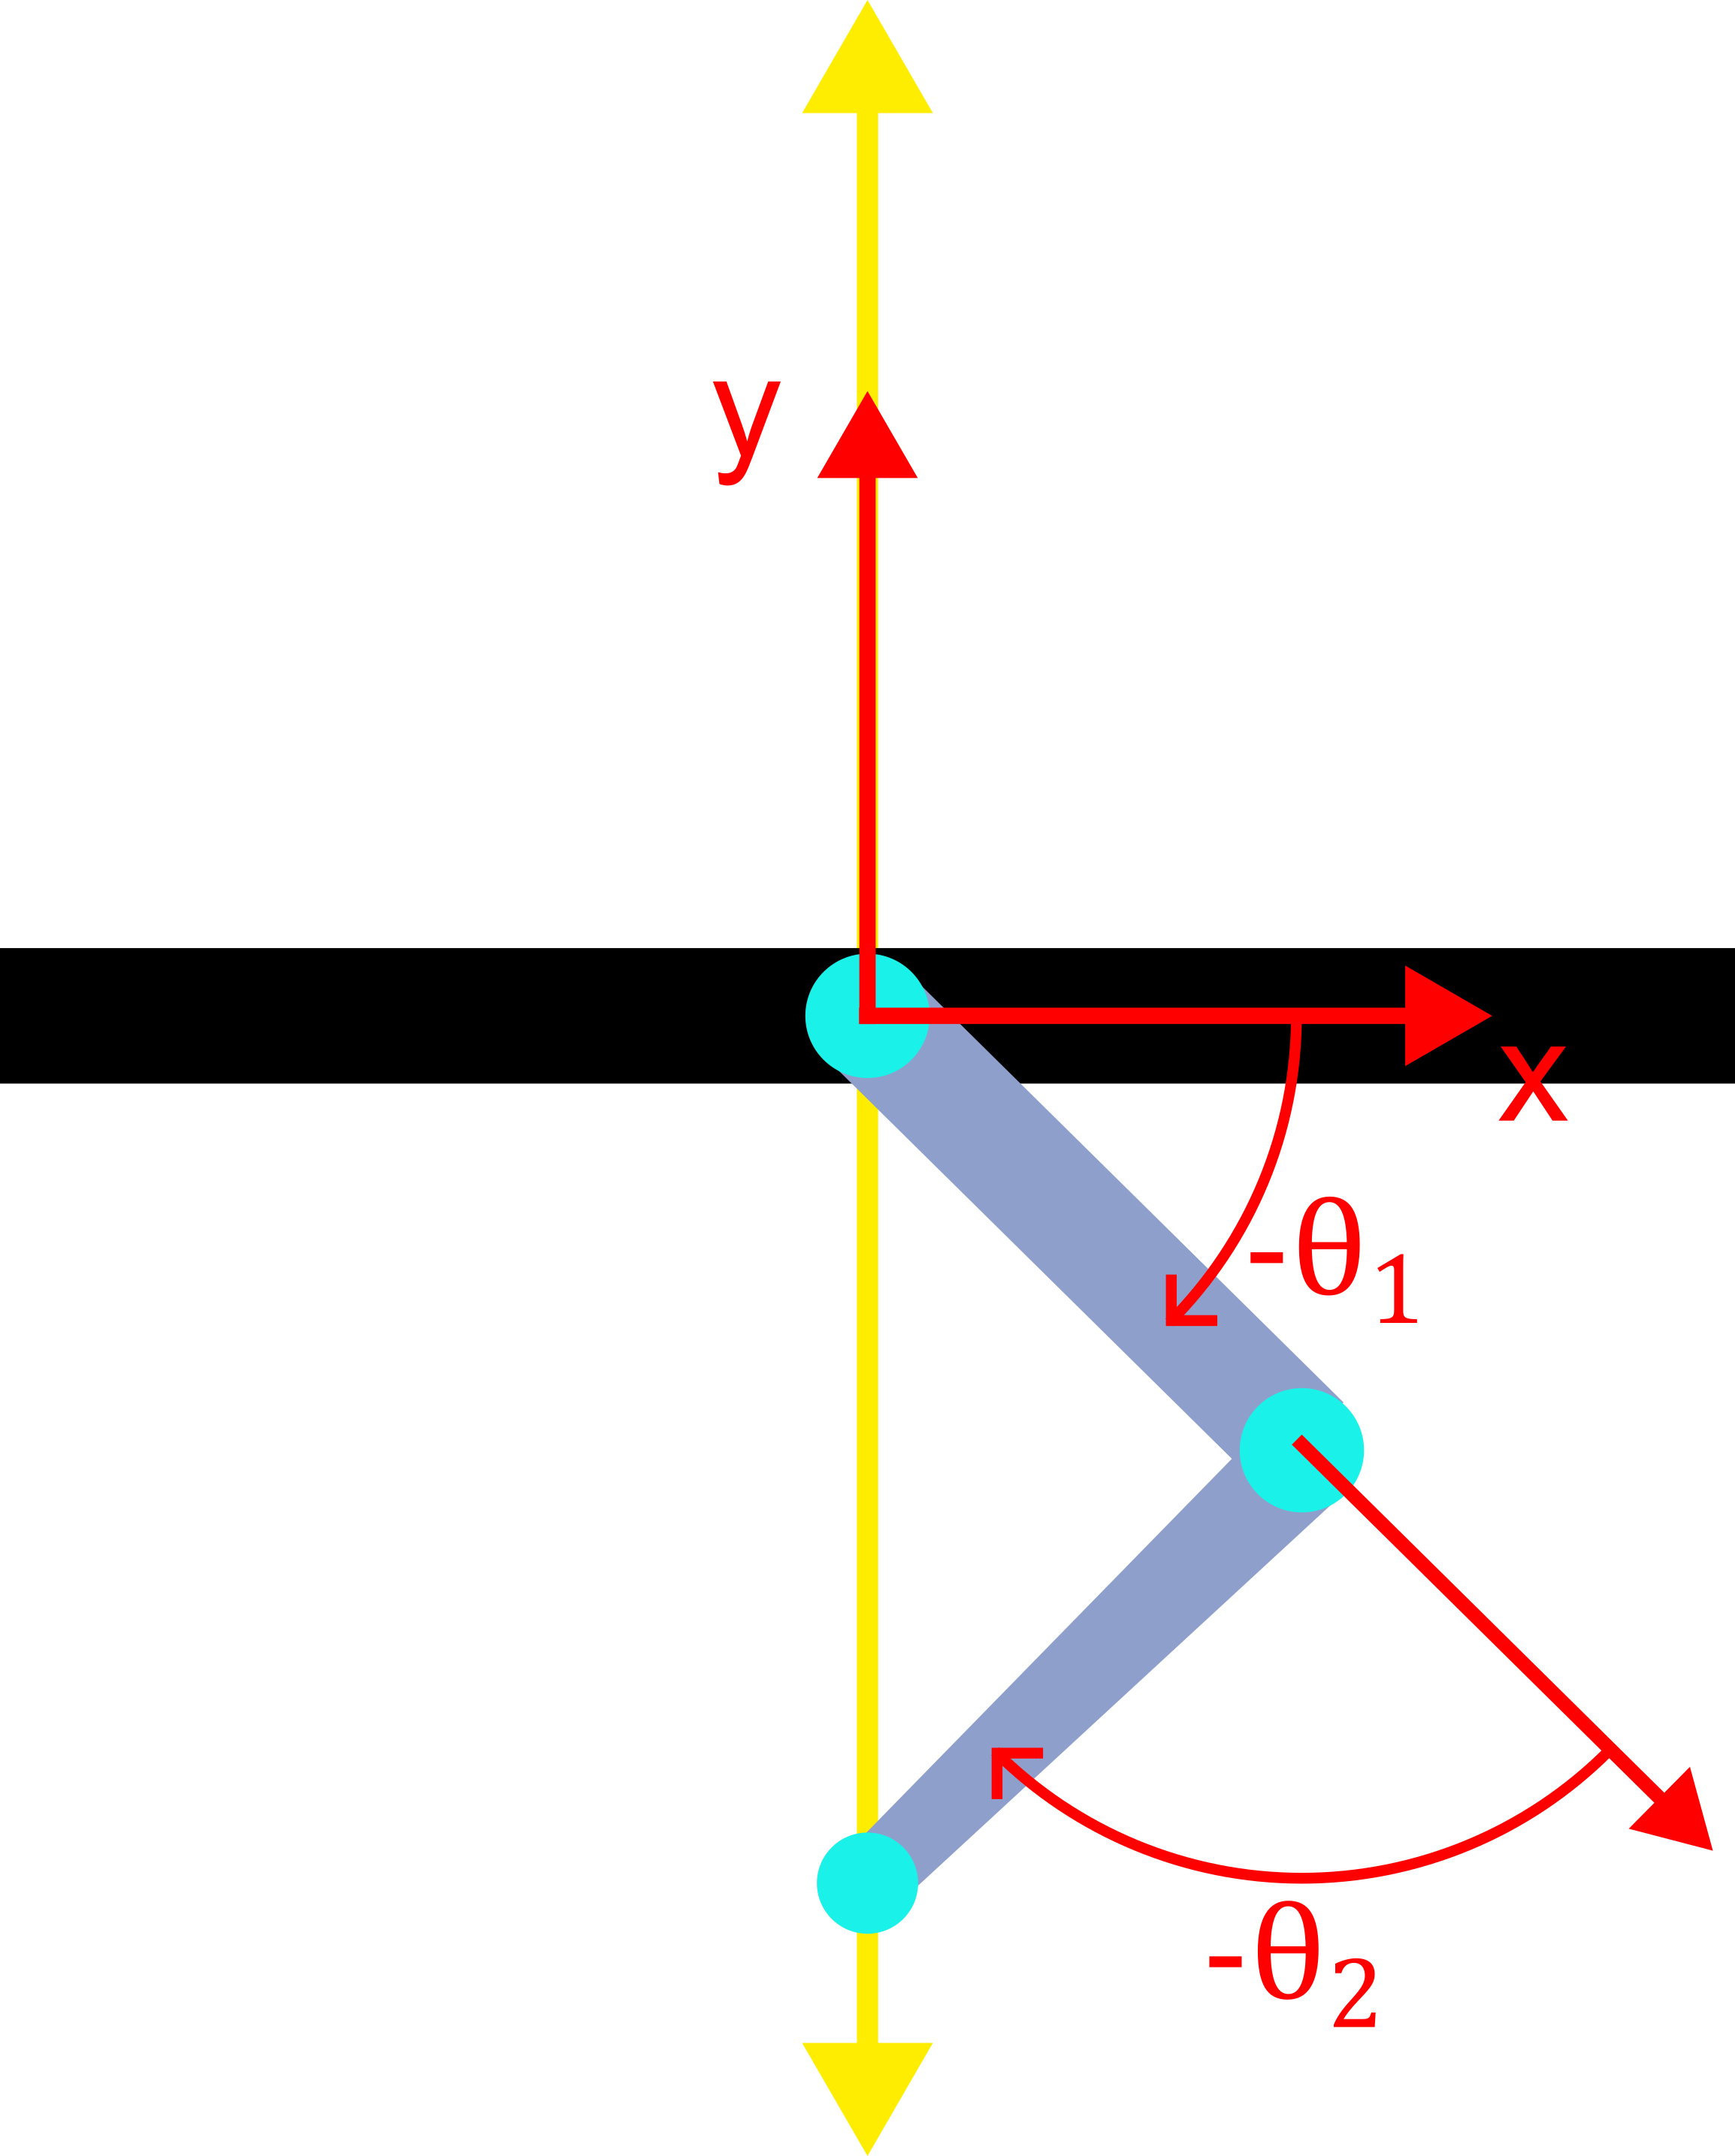
\includegraphics[width=0.75\textwidth]{Images/one_axis_jump.png}
    \caption{The manipulator corresponding to a vertical one leg jump.}
    \label{fig:vertical_manipulator}
\end{figure}

\begin{equation}
    \label{eq:2_link_manipulator}
    \begin{aligned}
        x_{\text{end}} &= L_1 \cos(\theta_1) + L_2 \cos(\theta_1 + \theta_2) \\
        y_{\text{end}} &= L_1 \sin(\theta_1) + L_2 \sin(\theta_1 + \theta_2)
    \end{aligned}
\end{equation}

\begin{equation*}
    \label{eq:jacobian_vertical_jump_leg}
    J = \begin{bmatrix} 
    -L_1 \sin(\theta_1) - L_2 \sin(\theta_1 + \theta_2) & -L_2 \sin(\theta_1 + \theta_2) \\
    L_1 \cos(\theta_1) + L_2 \cos(\theta_1 + \theta_2) & L_2 \cos(\theta_1 + \theta_2)
    \end{bmatrix}
\end{equation*}

\begin{figure}[h]
    \centering
    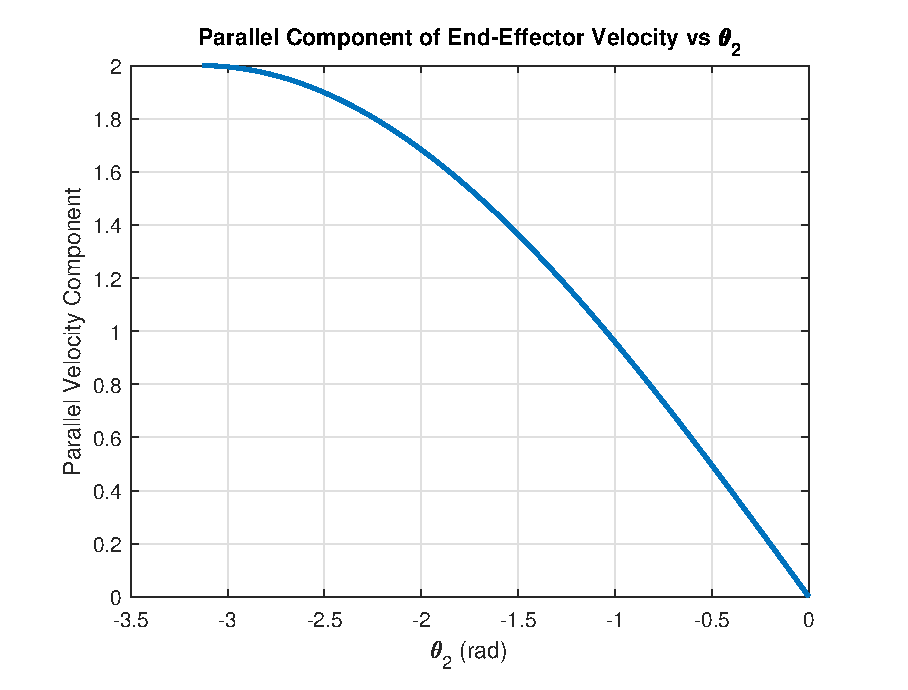
\includegraphics[width=\textwidth]{Images/vertical_paw_velocity.eps}
    \caption{Vertical Paw velocity as a function of knee angle.}
    \label{fig:vertical_jacobian_velocity}
\end{figure}

\subsection{Actuation Method Selection: Motors Only}
\label{sec:design_motor_only_jumps}
\begin{comment}
johanih@NTNU27686 MINGW64 ~/Documents/git/simscape_prosjektoppgave ((97ce13f...))
$ git log
commit 97ce13ff6832ea927897df16743914b9defbcdbf (HEAD)
Author: Johannes Ihle <johanih@ntnu.no>
Date:   Tue Oct 15 15:41:56 2024 +0200

    Updated everything according to status when sent message to Kostas
\end{comment} 

Initially, experiments were done utilizing motors alone. Due to the need for a light and strong motor, initially a series of AGF-RC motors were looked at, due to their high torque to weight ratio. As covered in section \ref{sec:motor_modeling}, a motor model consisting of a stall torque and a max velocity, with a linear decrease in max torque between these two, was chosen. For the AGF-RC motors, their provided stall torque and operating speed were used for the motor model parameters. Attempts were made to get more information about the motors' performance characteristics, but the supplier, AGF-RC, was unable to provide more detailed information. While extensive testing was done with various motors, the jumping performance was so far from acceptable that the idea was abandoned, and the full scope of the experiments are considered outside the scope of this report.

More details about the results of the motor only jumps can be found in section \ref{sec:results_motor_only_jumps}, but a brief overview of the reasoning involved will be given here. The most relevant of the motors chosen for these experiments was the A80BHP-H motor by AGF-RC, which was chosen because it had both the highest stall torque and operating speed of all the AGF-RC motors. Info about the A80BHP-H motor can be found in appendix \ref{appendix:A80_motor_info}. Attempts were made to identify motors in the same weight range with similar stall torques and operating speeds, but none were found. The experiments using the A80BHP-H were therefore, to a certain degree, considered an "optimistic estimate". Since no satisfactory results were achieved with the A80BHP-H motor, as discussed in section \ref{sec:results_motor_only_jumps}, it was decided to explore alternatives to motor-only actuation. 

The tests with the A80BHP-H motor were done by providing the knee motors with reference torques equal to their max torque, with the motor model limiting the resultant torque to more realistic values. Meanwhile, the hip joints were actuated according to the control law seen in equation \ref{eq:friction_cone_limit} to limit slipping. This control law is based on equation \ref{eq:force_torque_mapping}, as derived in section \ref{sec:force_torque_mapping}, combined with the theory on friction presented in section \ref{sec:contact_friction}. Equation \ref{eq:force_torque_mapping} is derived with an assumption of zero velocity/equilibria (TODO), an assumption that is obviously not valid for this dynamic jumping scenario. Despite this, very little slipping is observed in practice.   

\begin{align}
    N &= \text{Normal force} \\
    \mu &= \text{friction coefficient} = 0.8 \\
    \tau_{\text{friction cone limit}} &= J^T 
    \begin{bmatrix}
        N \mu \\
        0
    \end{bmatrix} \\
    \max(|\tau_{knee}|) &= \tau_{\text{friction cone limit}}
    \label{eq:friction_cone_limit}
\end{align}

Using this control law, jumping for variously dimensioned robots were attempted. As covered in section \ref{sec:results_motor_only_jumps}, none of them were satisfactory. Tests were eventually terminated, as no leg and body link length configuration was capable of jumping satisfactorily. By satisfactorily, it is meant that the robot center of mass cleared the ground by a distance more than twice that of the leg length, ie., if the legs are 20cm long, the center of mass should clear the ground by at least 40cm. 

For comparisons between this motor-only jumping and later spring+motor jumping, it is worth mentioning that the spring-motor jumping is done not with the A80BHP-H motors, but with weaker and slower motors, as well as with more realistic motor friction models. The reason the A80BHP-H motors were not used for the spring-motor jumping simulations, is that the motor supplier's website (AGF-RC) stated an operating travel range of 90 degrees. This was assumed to be correct, as other AGF-RC motors with stated operating ranges of 180 degrees have had actual mechanical limits of 220 degrees, so such a limitation was not considered out of the ordinary. For that reason, the motors initially purchased were not the A80BHP-H motors, and they are therefore not used for the rest of the experiments in this report. Later consultations with the supplier's website revealed conflicting information regarding the operating range of the A80BHP-H motor, and direct contact with the supplier revealed that the motor is in fact not limited to 90 degrees of travel. For this reason, potential use of the A80BHP-H motor for the spring-motor jumping is discussed in the future work section, section \ref{sec:future_work}. 


\subsection{Actuation Method Selection: Motors and Torsional Spring}

The next actuation method considered was to use a combination of motors and torsional springs, as this is the design we ended up choosing, a CAD model of this design can be seen in figure \ref{fig:assembly_CAD}. With this design, the knee motors are used to compress the torsional springs, once the knee joint reaches a desired angle, ie. has stored the desired amount of energy, the motors are turned off, and the springs accelerate the legs' joints quickly enough for the robot to take off. Results from simulations are presented in section \ref{sec:results:link_length_optimization}, but in short, jumping performance is superior to that of the motor-only jumps. For the spring-motor jumps, a friction model as derived in section \ref{sec:motor_friction_estimation} was used. Again, note the much weaker motor used in 

%The choice to use torsional springs in the knee only, rather than in both the hip and knee joints, was made in accordance to the goals stated in section \ref{sec:motivation}, ie. to make a robot that can jump, without excessively limiting its general utility as a quadruped. It is the belief of the authors that a normal walking gait, without having to compress or extend the torsional springs in the knees, could easily be achieved by introducing a mechanical slack that must be exceeded before the knee springs are compressed. This is however considered beyond the scope of this project, as this robot is only intended to jump. Comparatively, springs in the hips would affect things such as attitude stabilization

\subsection{Actuation Method Selection: Motors and Extension Spring}

In addition to the torsional spring design, attempts were made to design a leg utilizing an extension spring. The resulting design is shown in figure \ref{fig:extension_spring_CAD}. Although experiments akin to the ones done for torsional springs were done with comparable results, the extension spring design was ultimately abandoned. The reason for this was pure geometrical constraints, which are discussed in section \ref{sec:extension_spring_design}. Because the extension spring design was abandoned, the details surrounding the extension spring simulations and simulation results are considered outside the scope of this report.

\subsection{Hip Motor Strength Requirements}
\label{sec:hip_motor_dimensioning_test_design}

While the main purpose of the designed robot is to be proficient at jumping, the inclusion of torsional knee springs as a major part of the actuation method, and the subsequent lessened importance of the hip motors for jumping, complicated the choice of hip motors. For a conservative bound on on the torque and speed required for in air attitude stabilization
 \cite{finn_tarek_master} uses a heuristic of three 90-degree back-and-forth lateral swings per second as a benchmark. Although the purpose of our robot is not to do in-air attitude stabilization, this heuristic was partially utilized for verification that the hip motors were strong enough. More specifically, the robot body was fixed in space, and the robot's paws were set to be 1cm diameter spheres of iron (ie. with a density of 7800$\frac{kg}{cm^3}$, for a total mass of $\approx$32 g). The hip motor was then commanded to follow a trajectory according to the heuristic specified in \cite{finn_tarek_master}. The results of this simulation are presented in section \ref{sec:hip_motor_dimensioning_test}. While the paw masses used in \cite{finn_tarek_master} were 80g, the Eurepus robot's main body mass was also closer to 800g, compared to our body mass of approximately 300g. Our experimental paw masses of 32g were therefore considered appropriate, considering attitude stabilization is not strictly speaking a goal for the robot. 